
\documentclass[UTF8]{beamer}
\usetheme{Copenhagen}
%\usepackage{subfigure}
\usepackage{url}   % 网页链接
\usepackage{subcaption}
\usepackage{epstopdf}
\usepackage{graphicx}
%\usepackage[space,space,hyperref]{ctex}
\usepackage{ctex} %可以改成中文版
\captionsetup{font={small}}
\usetheme{Warsaw}
\author{Tong Wu}
\title{Introduction To Phase Retrieval}
\institute{Acknowledgment: this slide is based on Prof. Wen's and Dr. Stefano's lecture notes.}
\titlegraphic{
\includegraphics[height=1.5cm]{SYSULogo}}
\begin{document}
\frame{\titlepage}

%\tableofcontents
\begin{frame} \frametitle{介绍}
\begin{figure}[H]
\centering

    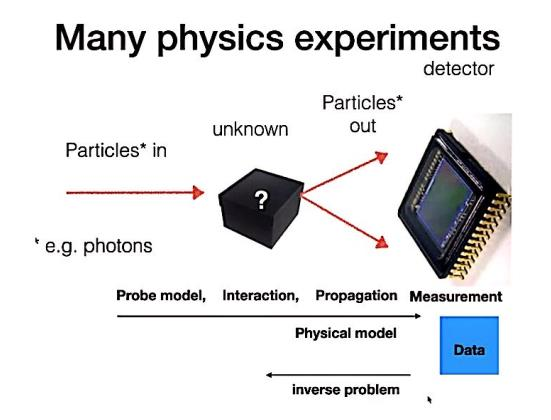
\includegraphics[width=1\linewidth]{../figures0/overall.jpg}  
   
\end{figure}
\end{frame}

\begin{frame} \frametitle{Missing phase problem}
\begin{figure}[H]
\centering

    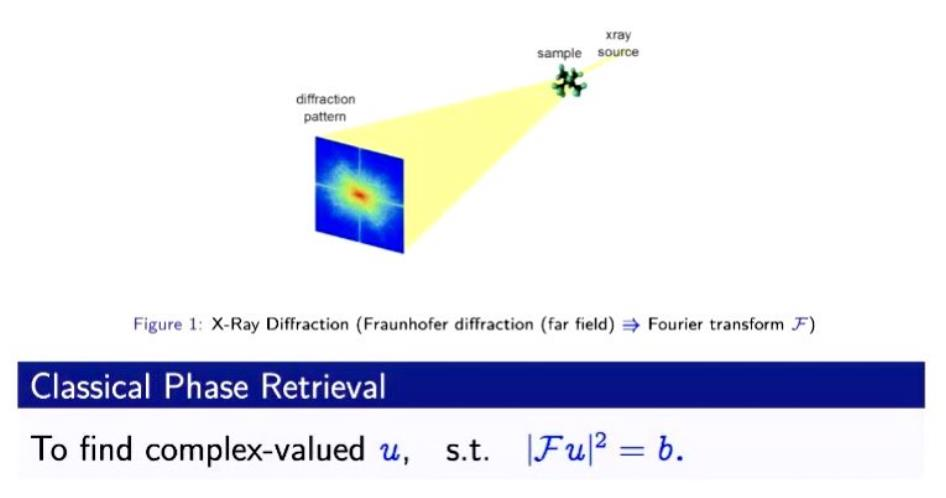
\includegraphics[width=1\linewidth]{../figures0/problem.jpg}  
   
\end{figure}
\end{frame}

\begin{frame} \frametitle{Phase and magnitude}
\begin{figure}[H]
\centering

    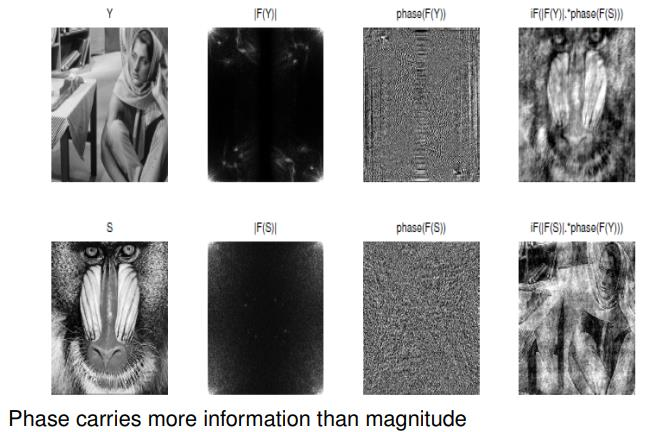
\includegraphics[width=1\linewidth]{../figures0/Phaseandmagnitude.jpg}  
   
\end{figure}
\end{frame}





\begin{frame}[c]\frametitle{Classical Phase Retrieval}
\begin{figure}[H]
\centering

    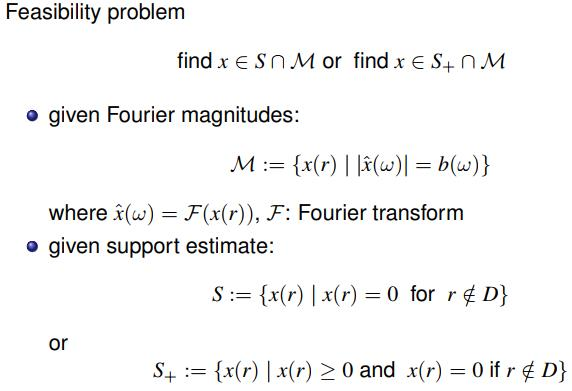
\includegraphics[width=1\linewidth]{../figures0/ClassicalPhaze.jpg}  
   
\end{figure}

\end{frame}

\begin{frame}[c]\frametitle{Error Reduction}


Alternating projection:
$$
x^{k+1}=\mathcal{P}_{\mathcal{S}} \mathcal{P}_{\mathcal{M}}\left(x^{k}\right)
$$
\begin{columns}

\begin{column}{0.5\textwidth}
\begin{enumerate}
\item(fit model) projection to $S$ :
$$
\mathcal{P}_{S}(x)=\left\{\begin{array}{cc}
x(r), & \text { if } r \in D \\
0, & \text { otherwise }
\end{array}\right.
$$
\item(fit data) projection to $\mathcal{M}$ :

$E = (|\mathcal{F}(x)|^2 - b)^2$
$\mathcal{P}_{\mathcal{M}}(x)=\mathcal{F}^{-1}(\hat{y})$, where $\hat{y}=\left\{\begin{array}{cc}b(\omega) \frac{\hat{x}(\omega)}{|\hat{x}(\omega)|}, & \text { if } \hat{x}(\omega) \neq 0 \\ b(\omega), & \text { otherwise }\end{array}\right.$

\end{enumerate}
\end{column}

\begin{column}{0.5\textwidth}
\begin{figure}
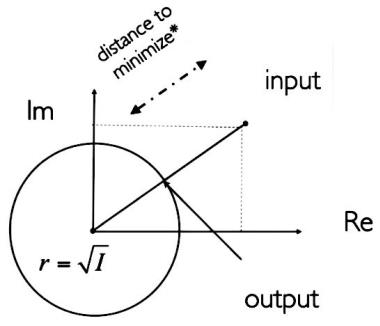
\includegraphics[width=1\linewidth]{../figures0/errorreduction.jpg}  
  \end{figure}
\end{column}

\end{columns}

\end{frame}


\begin{frame}[c]\frametitle{General sample method}

\begin{enumerate}


\item Phaseless measurements about $x_{0} \in \mathbf{C}^{n}$
$$
b_{k}=| a_{k}^* x_{0}|^{2}, \quad k \in\{1, \ldots, m\}
$$
\item Phase retrieval is feasibility problem
find $x_0$
s.t. $\quad | a_{k}^* x_{0}|^{2}=b_{k}, k=1, \ldots, m$

\item In the case above, $|\mathcal{F}x_0|^2 = b$,
we have:
$$
b_k = |f_k^*x_0|^2,  \quad k \in\{1, \ldots, n\}
$$
where $f_k^* \in C^{1 \times n}$ as a row vector  constructed from Fourier transform $\mathcal{F}$, to represent projection on frepuency element.
(Detail: 2D and 1D)

\end{enumerate}

\end{frame}

\begin{frame}[c]\frametitle{PhaseLift (C., Eldar, Strohmer, Voroninski, 2011)}
Lifting: $X=x x^{*}$
$$
b_{k}=| a_{k}^* x|^{2}=a_{k}^{*} x x^{*} a_{k}= Tr(a_{k}^{*} x x^{*} a_{k}) = Tr(a_{k} a_{k}^{*} x x^{*} )
=\left\langle a_{k} a_{k}^{*}, X\right\rangle
$$
Turns quadratic measurements into linear measurements $b=\mathcal{A}(X)$ about $x x^{*}$

\begin{columns}

\begin{column}{0.5\textwidth}
\begin{block}{Phase retrieval problem}
find $X$
s.t.
$$\begin{aligned}
&\mathcal{A}(X)=b \\
&X \succeq 0
, \operatorname{rank}(X)=1
\end{aligned}
$$
\end{block}
\end{column}

\begin{column}{0.5\textwidth}
\begin{block}{PhaseLift \& Relaxazion}
Min $Tr(X)$
s.t.
$$\begin{aligned}
&\mathcal{A}(X)=b \\
&X \succeq 0
\end{aligned}
$$
\end{block}
\end{column}

\end{columns}

\begin{alertblock}{Theorem (C. and Li (’12); C., Strohmer and Voroninski (’11))}

- $a_{k}$ independently and uniformly sampled on unit sphere

- $m \gtrsim n$

Then with prob. $1-O\left(e^{-\gamma m}\right)$, only feasible point is $x x^{*}$ $\{X: \mathcal{A}(X)=b$, and $X \succeq 0\}=\left\{x x^{*}\right\}$
\end{alertblock}
\end{frame}


\begin{frame}[c]\frametitle{Ptychographic Phase Retrieval}

%The theorem above serves as a benchmark result, but using Gaussian vectors as measurement vectors $a_k$ is not very realistic. For practical purposes, we prefer sets of measurement vectors that obey certain diffraction structure. 
For practical purposes, we may prefer sets of measurement vectors that obey certain diffraction structure. 
\begin{figure}[H]
\centering

    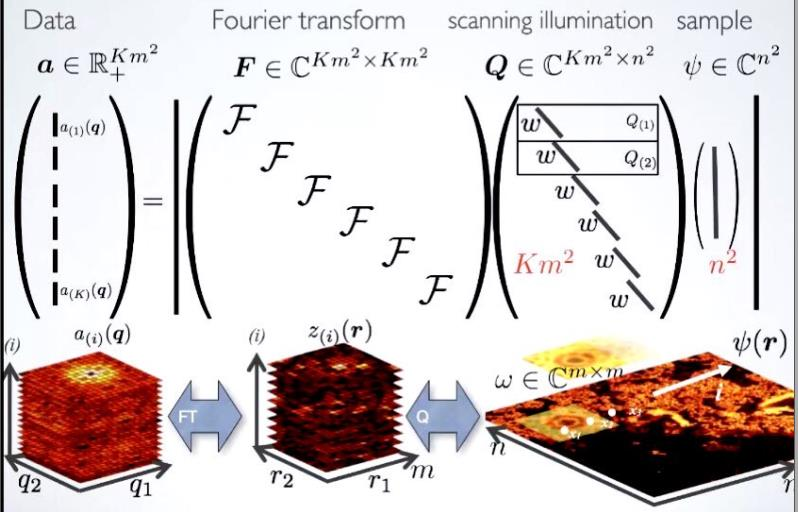
\includegraphics[width=1\linewidth]{../figures0/ptycho.jpg}  
   
\end{figure}

\end{frame}

\begin{frame}[c]\frametitle{Ptychographic Phase Retrieval}
\begin{equation}
\label{basic}
f_{j}=\left|\mathcal{F}\left( \mathcal{S}_{j} u  \circ \omega \right)\right|
\end{equation}

In a discrete setting, $u \in \mathbb{C}^{n^2}$ is a 2D image with $n \times n$ pixels, $\omega \in \mathbb{C}^{m^2}$ is a localized 2D probe with $m \times m$ pixels.

$f_{j} \in \mathbb{R}_{+}^{m^2}(\forall 1 \leq j \leq K)$ is a stack of phaseless measurements. Here $|\cdot|$ represents the element-wise absolute value of a vector, o denotes the elementwise multiplication, and $\mathcal{F}$ denotes the normalized 2 dimensional discrete Fourier transform. Each $\mathcal{S}_{j} \in \mathbb{R}^{m^2 \times n^2}$ is a binary matrix that crops a region $j$ of size $m^2$ from the image $u$.


\end{frame}



\begin{frame}[c]\frametitle{Ptychographic Phase Retrieval}

\begin{enumerate}
\item optimization problem
$$
\min \rho(u,w):=\sum_{j=1}^{K} \frac{1}{2}\left\|\left|\mathcal{F} ( \mathcal{S}_{j} u  \circ \omega)\right|-f_{j}\right\|_{2}^{2}
$$
\item Reformulation:
$$
\min \sum_{j=1}^{K} \frac{1}{2}\left\|\left|z_{j}\right|-f_{j}\right\|_{2}^{2} \text {, s.t. } z_{j}= \mathcal{A}_{j}(\omega, u):=\mathcal{F}\left(\omega \circ \mathcal{S}_{j} u\right),j=1... K
$$

\item Combine $j$:


$z = \mathcal{A}(\omega, u) := \left(\mathcal{A}_{1}^{T}(\omega, u), \mathcal{A}_{2}^{T}(\omega, u),..., \mathcal{A}_{K}^{T}(\omega, u)\right)^{T} 
\in \mathbb{C}^{ Km^2}$,

$f := (f_1^T,f_2^T, \ldots, f_K^T)^T$.

$$
\min \frac{1}{2}\left\|\left|z\right|-f\right\|_{2}^{2} \text {, s.t. } z= \mathcal{A}(\omega, u)
$$

\end{enumerate}


\end{frame}

\begin{frame}[c]\frametitle{ADMM}

Introduce $\Lambda \in C^{Km^2}$,
the corresponding augmented Lagrangian could be formulated as:

\begin{equation}
\begin{aligned}
&\Upsilon_{\beta}(\omega, u, z, \Lambda):=\frac{1}{2}\left\|\left|z\right|-f\right\|_{2}^{2}+\mathbb{I}_{\mathcal{X}_{1}}(\omega)+\mathbb{I}_{\mathcal{X}_{2}}(u)  \\
&+ \frac{\beta}{2}  \| z - \mathcal{A}(\omega, u) + \Lambda \|^{2} - \frac{\beta}{2}||\Lambda||^2 \\
\end{aligned}
\end{equation} 

$$
\begin{aligned}
\text {Step 1:} & \omega^{k+1}=\arg \min _{\omega} \Upsilon_{\beta}\left(\omega, u^{k}, z^{k}, \Lambda^{k}\right) \notag \\
 \text { Step 2: } & u^{k+1}=\arg \min _{u} \Upsilon_{\beta}\left(\omega^{k+1}, u, z^{k}, \Lambda^{k}\right) \notag \\ 
 \text { Step 3: } & z^{k+1}=\arg \min _{z} \Upsilon_{\beta}\left(\omega^{k+1}, u^{k+1}, z, \Lambda^{k}\right), \notag \\
\text { Step 4: } &
 \Lambda^{k+1}=\Lambda^{k}+\left(z^{k+1}-\mathcal{A}\left(\omega^{k+1}, u^{k+1}\right)\right)  \label{Lup}
\end{aligned}
$$

\end{frame}

\begin{frame}[c]\frametitle{Subproblems $\omega$ and $u$ }

$$
\begin{aligned}
&\omega^{k+1}=\arg \min _{\omega \in \mathcal{X}_{1}} \frac{1}{2}\left\|z^{k} + \Lambda^k -\mathcal{A}\left(\omega, u^{k}\right)\right\|^{2}\\
&=\arg \min _{\omega \in \mathcal{X}_{1}} \frac{1}{2}\left\|\hat{z}^{k}-\mathcal{A}\left(\omega, u^{k}\right)\right\|^{2}\\
\end{aligned}
$$
 
The close form solution of Step 1 is given as:
\begin{equation}
\omega^{k+1}=\operatorname{Proj}\left(\frac{ \sum_{j}\left(\mathcal{S}_{j} u^{k}\right)^{*} \circ [ \left(\mathcal{F}^{-1} \hat{z}_j^k\right) ]}{ \sum_{j}\mathcal{S}_{j} \left| u^{k} \right|^{2}} ; \mathcal{X}_{1}\right)
\label{omegaup}
\end{equation}  
Similarly we have:
\begin{equation}
\begin{aligned}
&\quad u^{k+1}=\operatorname{Proj}\left(\frac{\sum_{j} \mathcal{S}_{j}^{T}\left(\left(\omega^{k+1}\right)^{*} \circ \mathcal{F}^{-1} \hat{z}_{j}^{k}\right)}{\sum_{j}\left(\mathcal{S}_{j}^{T}\left|\omega^{k+1}\right|^{2}\right)} ; \mathcal{X}_{2}\right) \text { . }
\end{aligned}
\label{uup}
\end{equation}
Here $S_j^T$ is an operator mapping its augment to the target position $j$ in image $u$. 


\end{frame}

\begin{frame}[c]\frametitle{Subproblem $z$ }
 $$
  \quad z^{k+1}=\arg \min _{z} \frac{1}{2}\left\|\left|z\right|-f\right\|_{2}^{2} +\frac{\beta}{2}\left\|z^+-\mathcal{A}\left(\omega^{k+1}, u^{k+1}\right)\right\|^{2}
  $$
 $$
 = \arg \min _{z} \sum_{x,y,j} [\frac{1}{2} (  |z(x,y,j)|^2 - f(x,y,j) )^2 +
  \frac{\beta}{2}||z(x,y,j) - z^+(x,y,j)||^2 ]
 $$
 
 where $z^+ = \mathcal{A}\left(\omega^{k+1}, u^{k+1}\right) - \Lambda^{k}$
 
 For any fixed $x,y,j$, the problem can be seen as:
 
 $$
 z^*(x,y,j) = \arg \min_{z_{x,y,j} \in \mathbb{C}^{r}} \frac{1}{2} ( |z_{x,y,j}| - f_{x,y,j} )^2
 + \frac{\beta}{2} |z_{x,y,j} - z_{x,y,j}^+|^2
 $$
 
\end{frame}



\begin{frame}[c]\frametitle{Subproblem $z$ }
 Notice that for fixed $|z_{x,y,j}|$, the first term in expression is fixed. To optimize the second term, we should always choose $z_{x,y,j}$ with the same direction as $z_{x,y,j}^+$. So we have: $\dfrac{z}{|z|} = \dfrac{z^+}{|z^+|}$, $|z_{x,y,j} - z_{x,y,j}^+|^2 = (|z_{x,y,j}| - |z_{x,y,j}^+|)^2$,
 $
   z(x,y,j) = |z_{x,y,j}|\dfrac{z^+(x,y,j)}{|z_{x,y,j}^+|}
 $
 To determine $z_{x,y,j}$, we only need to determine $|z_{x,y,j}|$. Denote it as $a$.
 $$
 |z_{x,y,j}|^* = \arg \min_{a \in \mathbb{R}} \frac{1}{2}(a - f_{x,y,j})^2 + \dfrac{\beta}{2}
 (a - |z_{x,y,j}^+|)^2
 = \dfrac{f_{x,y,j} + \beta |z_{x,y,j}^+|}{1 + \beta}
 $$
 The  close form solution of Step 3 is given as:
 
 \begin{equation}
 z^{k+1} = \dfrac{z^+ \dfrac{f}{ |z^+|} + \beta z^+}{1+\beta},
 \label{zup}
 \end{equation}
\end{frame}

\begin{frame}[c]\frametitle{New problem: partially coherent}

\begin{figure}
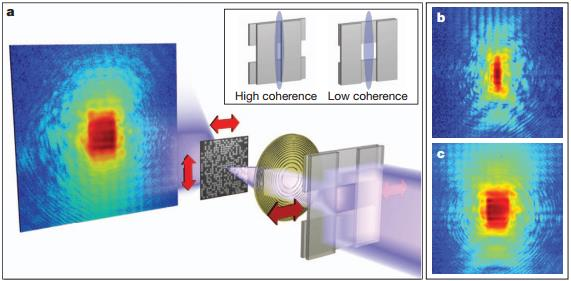
\includegraphics[width=1\linewidth]{../figures0/partially.jpg}  
  \end{figure}




\end{frame}

\begin{frame}[c]\frametitle{Partially coherent model: a general one}
\framesubtitle{Thibault, Pierre, and Andreas Menzel. "Reconstructing state mixtures from diffraction measurements." Nature 494.7435 (2013): 68-71.}



\structure{Blind ptychography model + quantum state tomography\footnote{\url{https://homepage.univie.ac.at/reinhold.bertlmann/pdfs/T2_Skript_Ch_9corr.pdf} Many symbols in quantum mechanics are included here.}.}

Phobe $w$ is assumed to be in mixed state to represent partially coherent effect.

\begin{equation}
\label{model:sep} 
\begin{aligned}
&\mbox{Find } u, r \mbox{ $w_k$   }s.t. \\
&f_{p c, j}=\sum_{k=1}^r \left|\mathcal{F}\left( \mathcal{S}_{j} u \circ \left(\omega_k\right) \right)\right|^{2}  
\end{aligned}
\end{equation}




\end{frame}




\begin{frame} \frametitle{Partially coherent model: a general one}

Denote $O_j \in C^{m^2 \times m^2}$ as a (diagonal) matrix to represent linear transform to $w$, s.t. $\mathcal{S}_{j} u \circ \omega = O_j w$. Denote $f_q^* \in C^{1 \times m^2}$ as a row vector  constructed from Fourier transform $\mathcal{F}$, to represent projection on frepuency element. Construct measurement matrix $ \mathcal{I}_{j \mathbf{q}} = O_j^*f_qf_q^*O_j$ and density matrix $\rho$, we get another form(actually a natural one in quantum state tomography) of the model:


\begin{equation}
\label{lift}
\begin{aligned}
&\mbox{Find } u,\rho,s.t.\\
&f_{pc,j}(q) = Tr(\mathcal{I}_{j \mathbf{q}} \rho ) (1\leq j \leq K)\\
&\rho \mbox{ is positive semi-definite, with rank}\leq r 
\end{aligned}
\end{equation}



\end{frame}



\begin{frame} \frametitle{Partially coherent model: a general one}
Next, we will explain the derivation of this form.

 Simple calculation process:
$$
f_{pc,j}(q) = |f_q^*O_j w|^2 = (f_q^*O_j w)^*(f_q^*O_j w) = w^*(O_j^*f_qf_q^*O_j)w
$$
$$
=Tr[w^*(O_j^*f_qf_q^*O_j)w]=Tr[(O_j^*f_qf_q^*O_j) (ww^*)]
$$
$$
=Tr(  \mathcal{I}_{j \mathbf{q}} \rho ),
\rho = ww^*
$$

\end{frame}




\begin{frame} \frametitle{Connection to a particular model}

Continuous setting:

\begin{equation}
f_{p c, j}(q) = \int\left|\mathcal{F}_{x \rightarrow q}\left(\mathcal{S}_{j} u(x) \omega(x-y)\right)\right|^{2} \kappa(y) \mathrm{d} y
\end{equation}

Discrete setting:

\begin{equation}
f_{p c, j}=\sum_{i} \kappa_{i}\left|\mathcal{F}\left( \mathcal{S}_{j} u \circ \left(\mathcal{T}_{i} \omega\right) \right)\right|^{2}
\label{model:target}
\end{equation}

 We put the $\kappa_{i}$ inside:
\begin{equation}
f_{p c, j}=\sum_{i} \left|\mathcal{F}\left( \mathcal{S}_{j} u \circ \left( \sqrt{\kappa_{i}}\mathcal{T}_{i} \omega\right) \right)\right|^{2}
=
\sum_{i} \left|\mathcal{F}\left( \mathcal{S}_{j} u \circ \left( \hat{\omega}_i\right) \right)\right|^{2}
\end{equation}
Multiple modes $\hat{w}_i$ are produced by shifted $w$. Then we can construct density matrix and use truncated SVD to get a low-rank approximation. Then it is exactly \eqref{model:sep}
$$
\rho = \sum_i \hat{w}_i \hat{w}_i^* \approx \sum_{k=1}^{r} w_k w_k^* 
$$

\end{frame}

\begin{frame} \frametitle{Performance Metrics}

\begin{enumerate}
\item Relative error $err$ and signal-to-noise ratio $snr$
$$
err^k = \dfrac{|| c u^k - u_{true} ||_F  }{||c u^k||_F}, c = \frac{sum(u_{true} \circ \overline{u^k}) }{||u^k||_F^2}
$$
$$
snr^k = -20\log_{10}(err^k)
$$
$|| \cdot ||_F$ is the Frobenius norm. $err$ measures the difference between a reconstructed image and the groundtruth image. $c$ is an estimated scale factor, and $sum$ means the sum of all elements in the target matrix. 

\item R-factor $R$

Let $zz = \mathcal{A}_{j}\left(\omega^{k}, u^{k}\right)$
$$
R^{k}:=\frac{\left\| |zz|-f\right\|_{1}}{\|f\|_{1}}
$$
$R$ measures the difference between the reconstruction diffraction stacks and groundtruth stacks $f$. 

%We don't always know $u_{true}$, $Y$ is the only input data for our algorithm, and R-factor can be used to verify the convergence.

%\item signal-to-noise ratio $SNR$
%$$
%SNR^k = -20\log_{10} (\dfrac{|| u^k - u_{true} ||_F  }{|| u_{true}||_F})
%$$


\end{enumerate} 


\end{frame}


\begin{frame} \frametitle{Simulation Experiment}

$Dist=8$, regular grid, viberation model, and $\kappa$ is a guassian kernel with $\sigma = (15,15)$. $\beta=0.05$ is chosen as algorithm parameter for ADMM.

\begin{figure}[H]
\centering
\begin{subfigure}{1\textwidth}
    \centering
    % include first image
    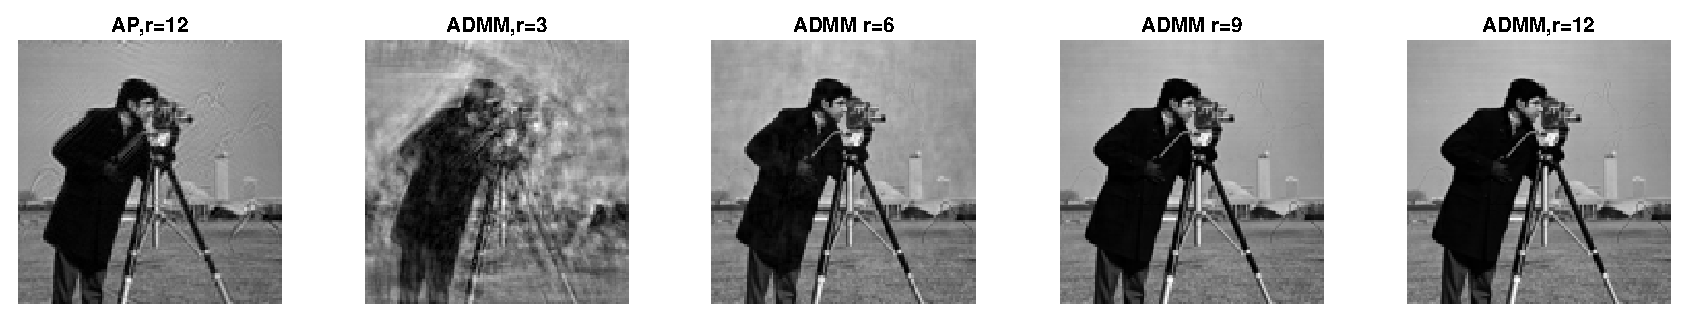
\includegraphics[width=0.9\linewidth]{../figures/modes_u.eps}  
   \caption{Amplitude}
    \label{fig:modes_u}
 \end{subfigure}
 \begin{subfigure}{1\textwidth}
    \centering
    % include second image
    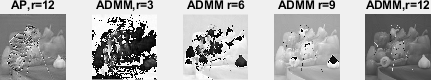
\includegraphics[width=.9\linewidth]{../figures/modes_u_phaze.png}  
    %\caption{Put your sub-caption here}
    \caption{Phase}
    \label{fig:modes_u_phaze}
 \end{subfigure}
 
    \label{fig:modes_images}

 \end{figure}


\end{frame}

\begin{frame} \frametitle{Simulation Experiment}
 \begin{figure}[H]
 \begin{subfigure}{.5\textwidth}
    \centering
    % include first image
    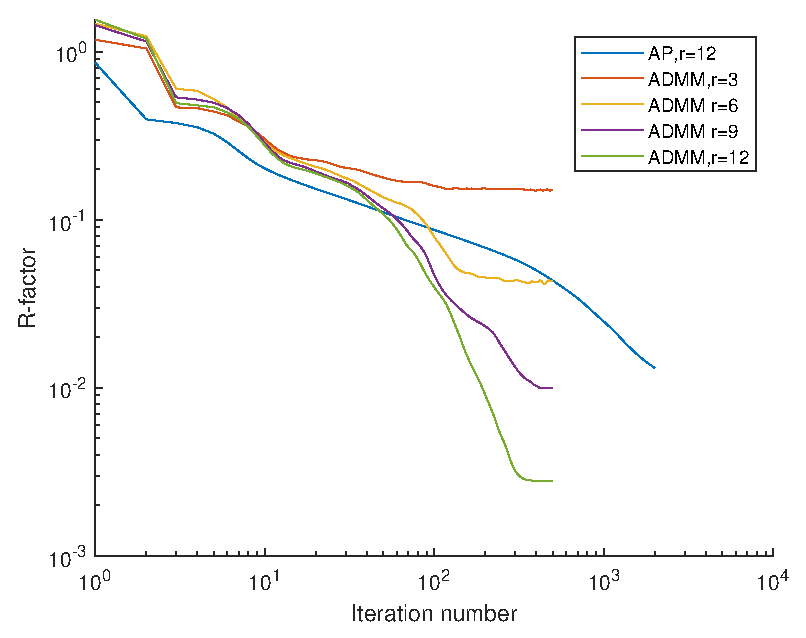
\includegraphics[width=1\linewidth]{../figures/modes_R.eps}  
    %\caption{}
    \label{fig:modes_R}
 \end{subfigure}
 \begin{subfigure}{.45\textwidth}
    \centering
    % include second image
    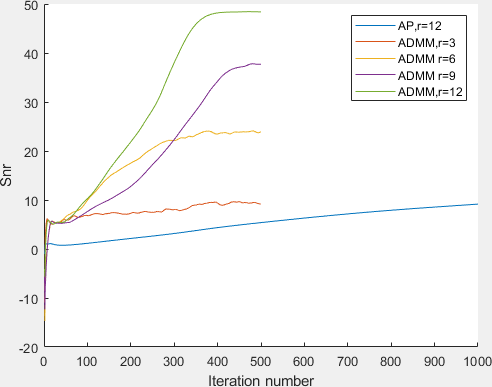
\includegraphics[width=1\linewidth]{../figures/modes_snr.png}  
    %\caption{Put your sub-caption here}
    \label{fig:modes_snr}
 \end{subfigure}
 \caption{R and snr. }
 \label{fig:noise}
 \end{figure}


%We first compare $snr$ and $R$ for reconstructed images using a different number of modes. When the number of modes increases, the $R-factor$ decreases, and the $snr$ increases. That indicates that the quality of the reconstructed image increases.

%The $R$ for 3,6,9,12 modes using ADMM algorithm are stable after 500 iterations at 0.15, 0.042, 0.0099, 0.0028, respectively, when $R$ for AP does not converge after 2000 iterations.

%similar k*f
\end{frame}

\begin{frame} \frametitle{Simulation Experiment}
\begin{figure}[H]
\centering
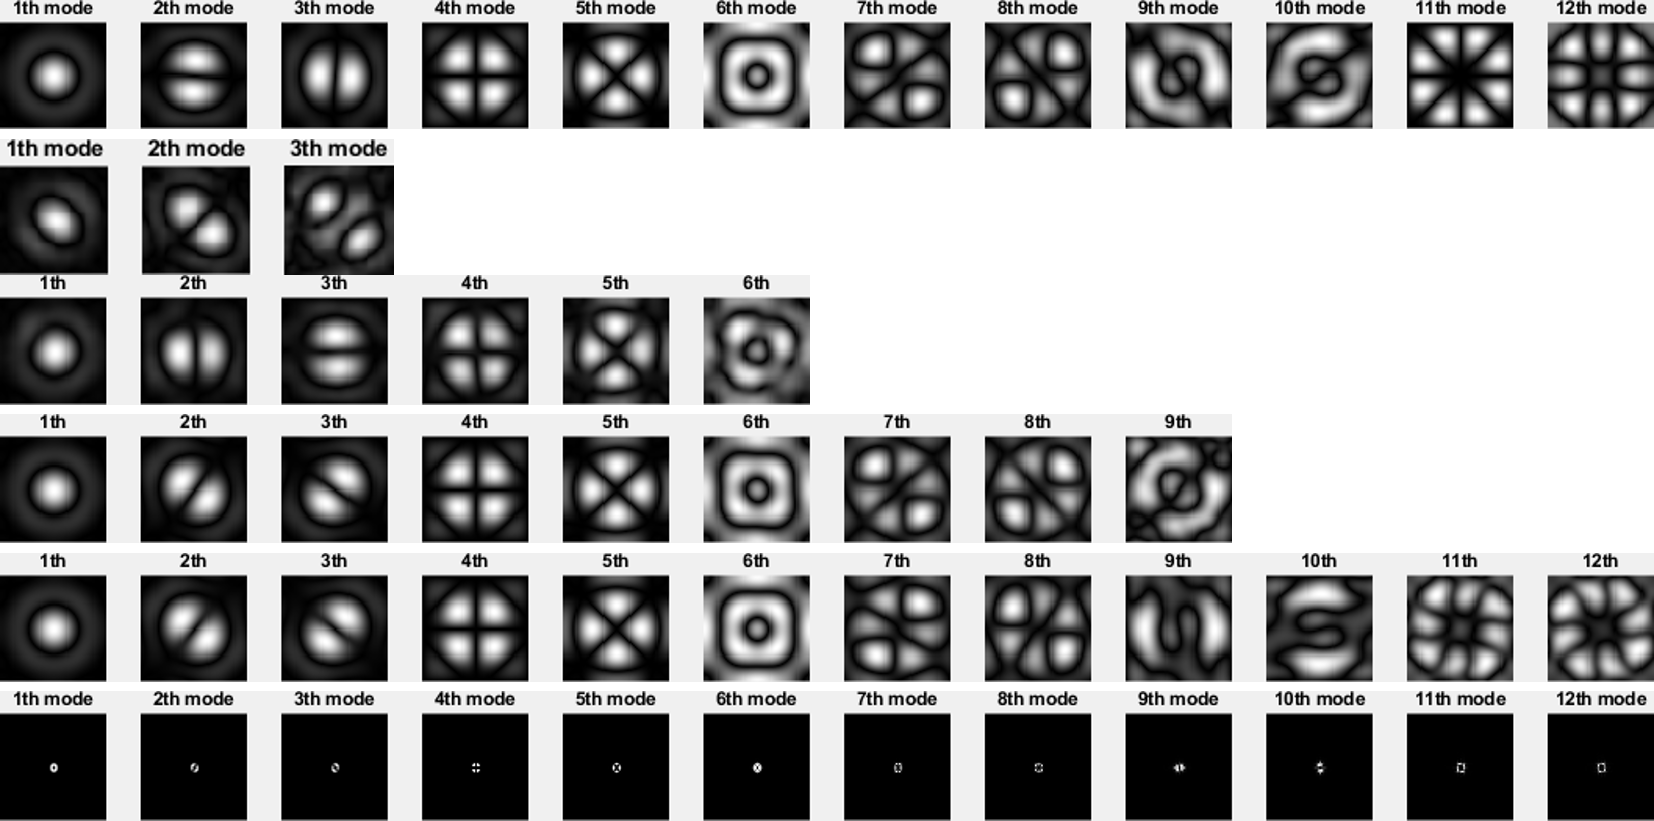
\includegraphics[width=1\linewidth]{../figures/modes_combine}
\caption{Mode pattern. The first row represents the standard mode pattern. And the last two rows represent the mode pattern for 12 modes. Mode patterns are in the time domain except that the last row is in the frequency domain.}
\label{fig:modescombine}
\end{figure}

%Standard mode pattern is obtained through performing SVD on standard density matrix generated from the model and extracting the first 12 modes. As shown in Figure \ref{fig:modescombine}, our algorithm can generally catch the main modes and get an optimal approximation.

\end{frame}


\begin{frame} \frametitle{Discussion}

Generally find a low-rank matrix $\rho$ based on \eqref{model:sep}, which has
special structures based on particular models like \eqref{model:target}

Two possible ways:

\begin{enumerate}

\item \structure{Transfer existing algorithms}:  

related to Low-rank Matrix Recovery

\item \structure{Exploit new structure}:

Rank-1 Matrix + vibration kernel $\kappa$ $\rightarrow$ matrix $\rho$

The rank-1 matrix comes from the main mode (Bessel).

Why approximated low-rank?

Why special patterns for modes decomposed from $\rho$? 
\end{enumerate}





\end{frame}

\begin{frame} \frametitle{Example: Guassian $\kappa$ (15 15)}
\begin{figure}[H]
\centering
%\caption{}
\begin{subfigure}{1\textwidth}
    \centering
    % include first image
    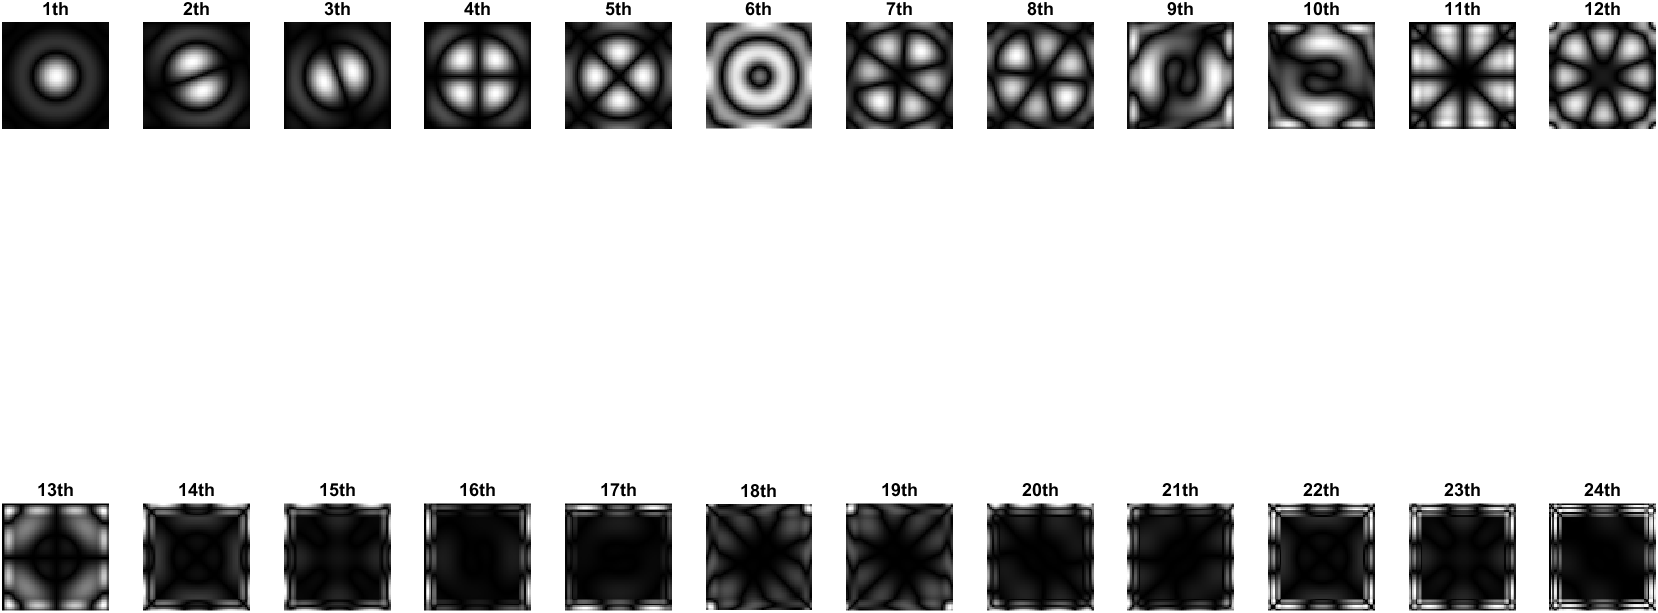
\includegraphics[width=0.9\linewidth]{../figures/ex_gu15_15.png}  
   %\caption{Ideal modes}
    \label{fig:modes_u}
 \end{subfigure}
 \begin{subfigure}{1\textwidth}
    \centering
    % include second image
    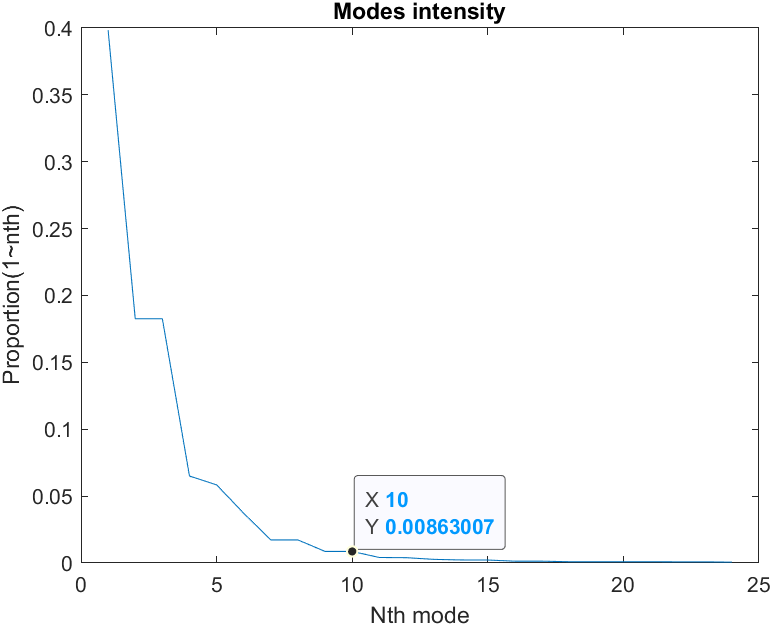
\includegraphics[width=.5\linewidth]{../figures/ex_gu15_15_s.png}  
    %\caption{Put your sub-caption here}
    %\caption{Singular value distribution}
    \label{fig:modes_u_phaze}
 \end{subfigure}
 
    \label{fig:modes_images}

 \end{figure}
\end{frame}


\begin{frame} \frametitle{Example: Retangular $\kappa$ (20 20)}
\begin{figure}[H]
\centering
\begin{subfigure}{1\textwidth}
    \centering
    % include first image
    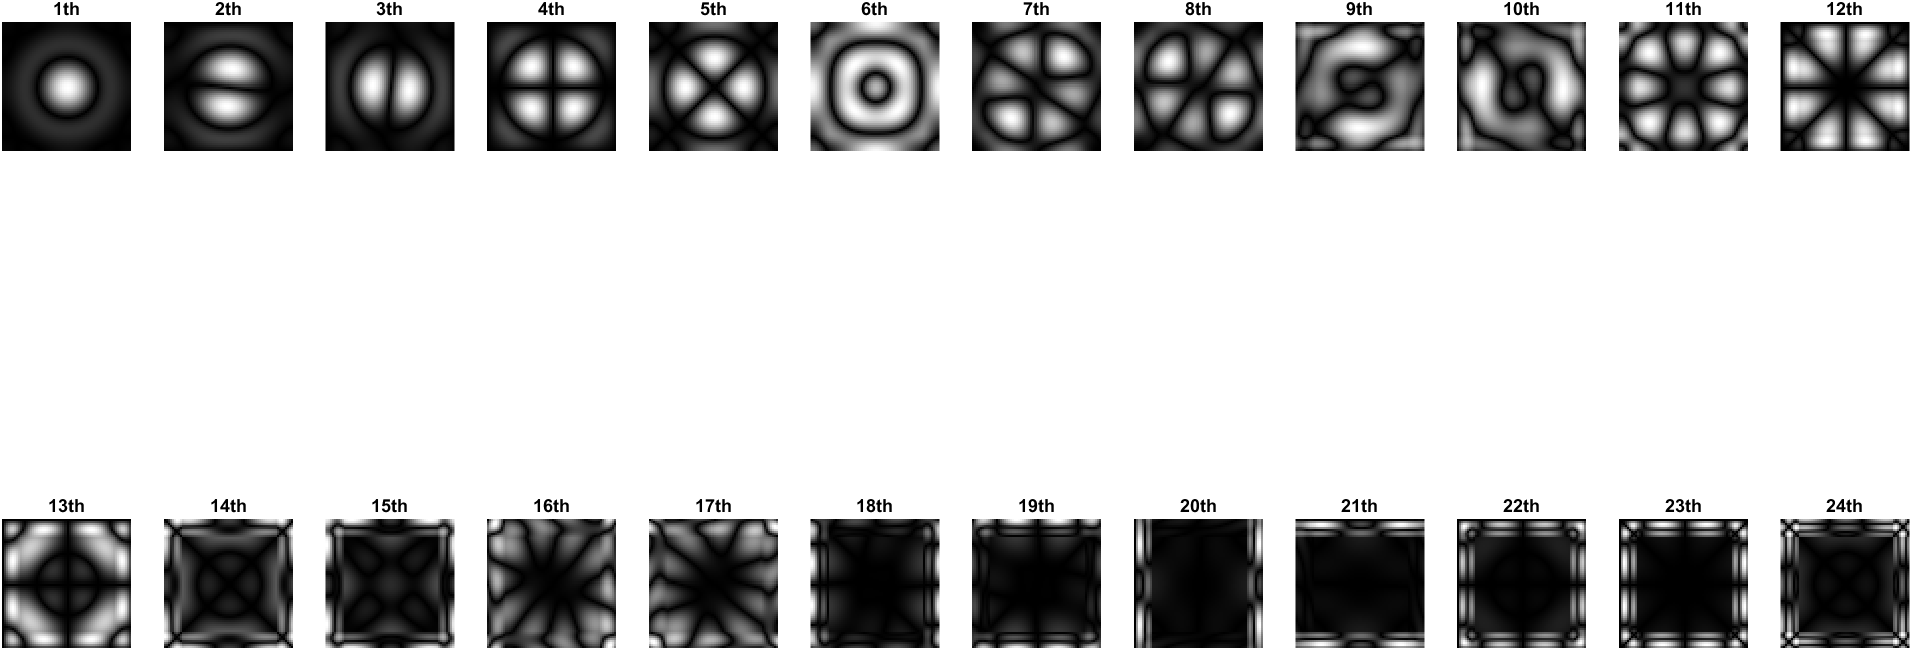
\includegraphics[width=0.9\linewidth]{../figures/ex_ave20.png}  
   %\caption{Ideal modes}
    \label{fig:modes_u}
 \end{subfigure}
 \begin{subfigure}{1\textwidth}
    \centering
    % include second image
    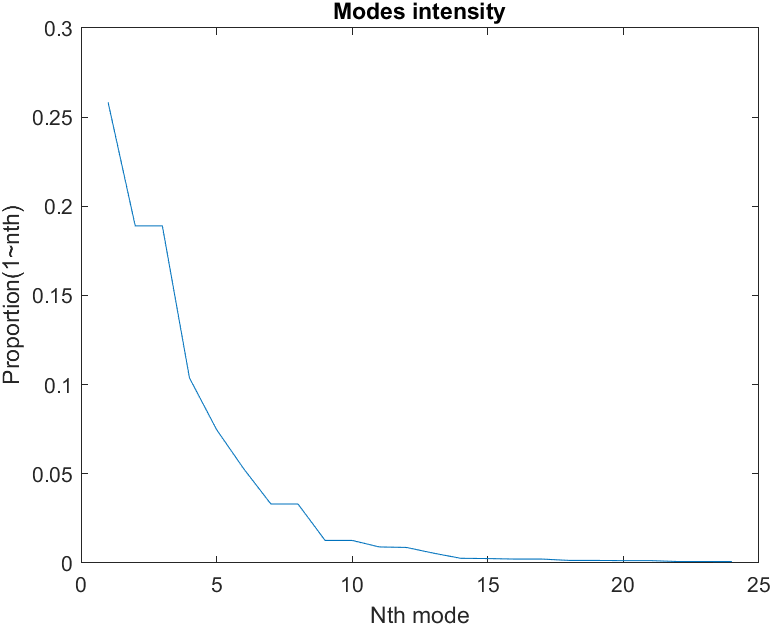
\includegraphics[width=.5\linewidth]{../figures/ex_ave20_s.png}  
    %\caption{Put your sub-caption here}
    %\caption{Singular value distribution}
    \label{fig:modes_u_phaze}
 \end{subfigure}
 \end{figure}
\end{frame}

\begin{frame} \frametitle{Example: Guassian $\kappa$ (4 0)}
\begin{figure}[H]
\centering
\begin{subfigure}{1\textwidth}
    \centering
    % include first image
    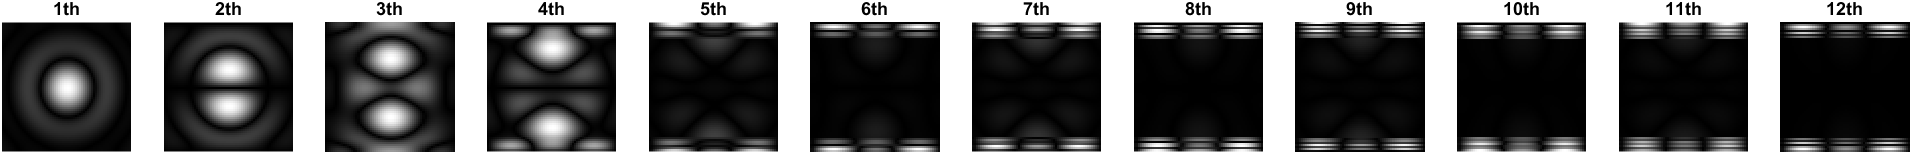
\includegraphics[width=0.9\linewidth]{../figures/ex_gu4_0.png}  
   %\caption{Ideal modes}
    \label{fig:modes_u}
 \end{subfigure}
 \begin{subfigure}{1\textwidth}
    \centering
    % include second image
    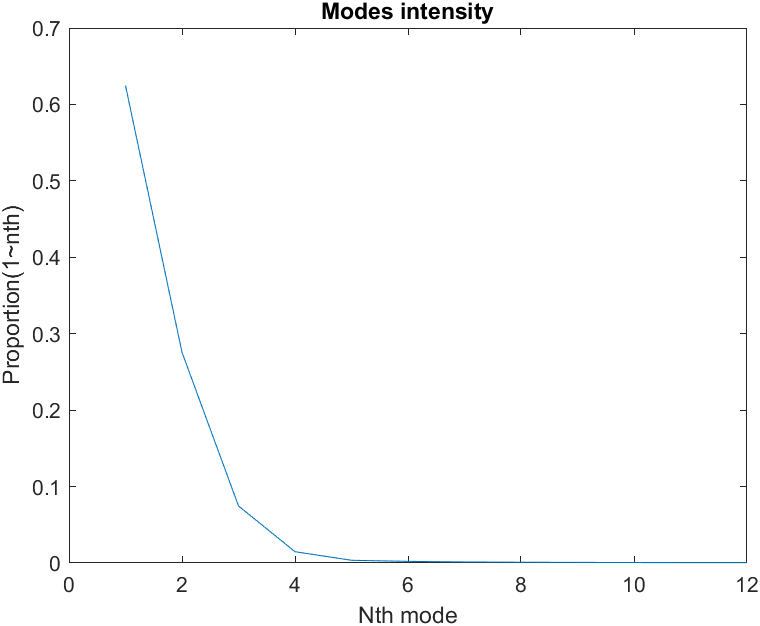
\includegraphics[width=.5\linewidth]{../figures/ex_gu4_0_s.png}  
    %\caption{Put your sub-caption here}
    %\caption{Singular value distribution}
    \label{fig:modes_u_phaze}
 \end{subfigure}
 \end{figure}
\end{frame}

\begin{frame} \frametitle{Example: Motion $\kappa$ (len=20,theta=45)}
\begin{figure}[H]
\centering
\begin{subfigure}{1\textwidth}
    \centering
    % include first image
    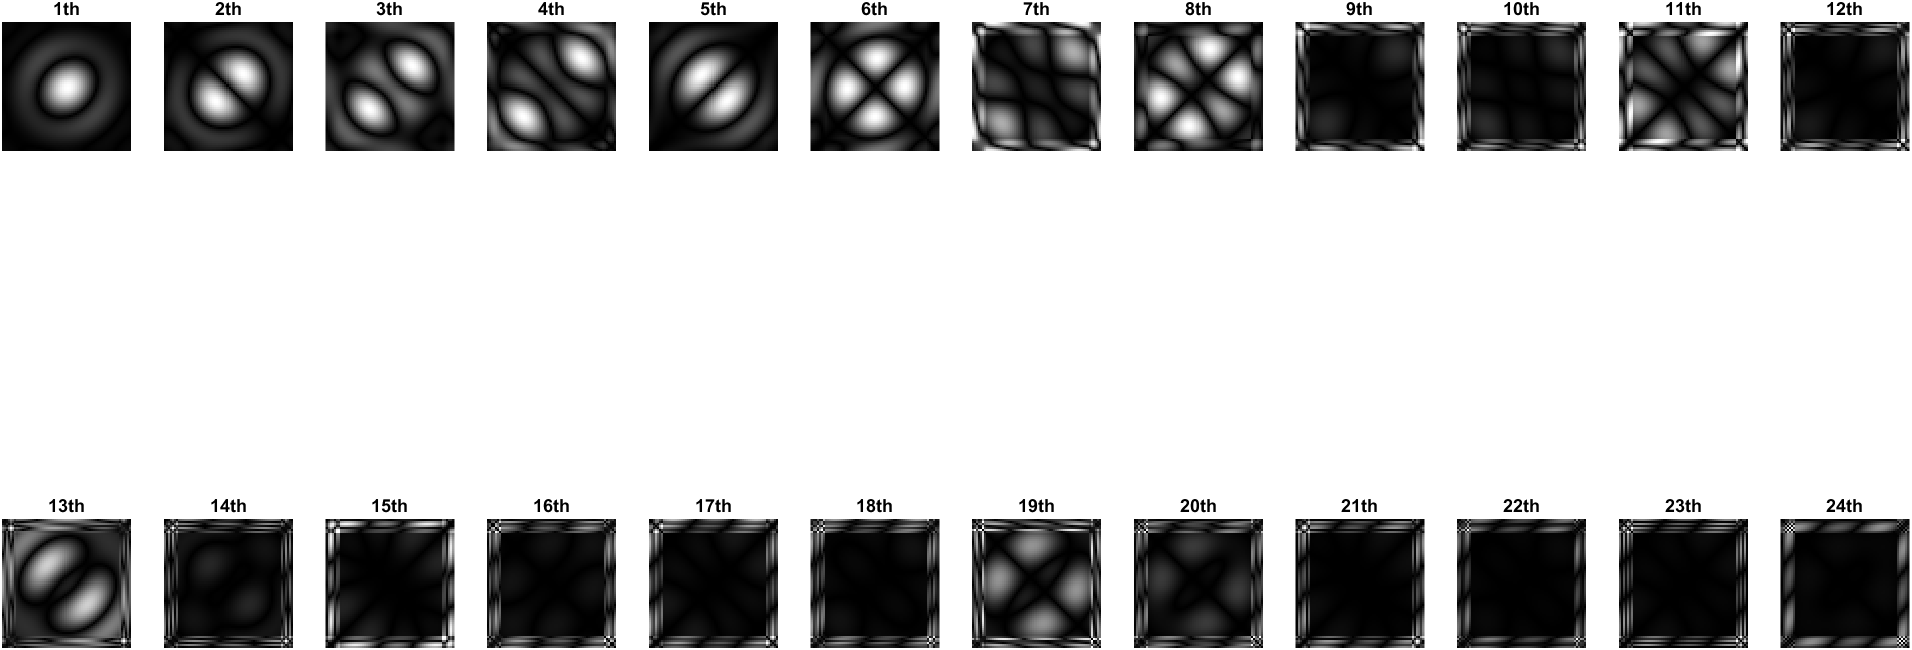
\includegraphics[width=0.9\linewidth]{../figures/ex_motion.png}  
   %\caption{Ideal modes}
    \label{fig:modes_u}
 \end{subfigure}
 \begin{subfigure}{1\textwidth}
    \centering
    % include second image
    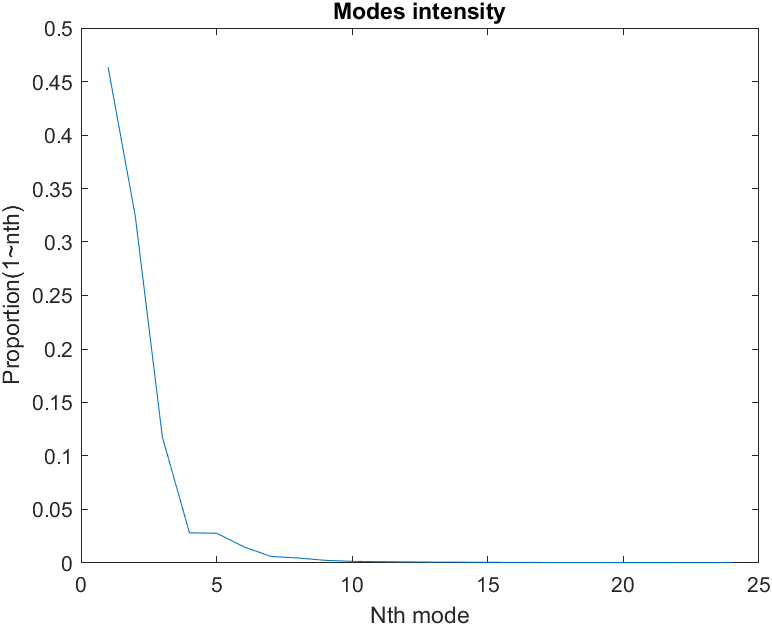
\includegraphics[width=.5\linewidth]{../figures/ex_motion_s.png}  
    %\caption{Put your sub-caption here}
    %\caption{Singular value distribution}
    \label{fig:modes_u_phaze}
 \end{subfigure}
 \end{figure}
\end{frame}

\begin{frame} \frametitle{Gradient decomposition}
\begin{equation}
f_{p c, j}(q) = \int\left|\mathcal{F}_{x \rightarrow q}\left(\mathcal{S}_{j} u(x) \omega(x-y)\right)\right|^{2} \kappa(y) \mathrm{d} y
\end{equation}
Expand $\omega$
\begin{figure}[H]
\centering

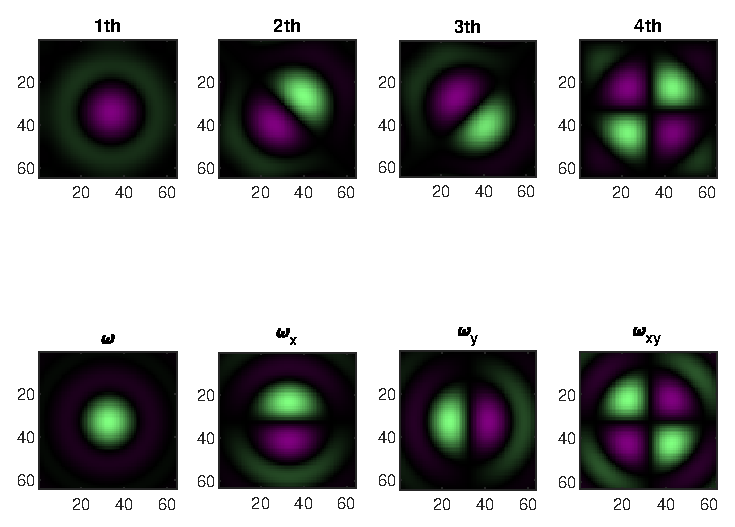
\includegraphics[width=0.8\linewidth]{../figures/gradients.eps}  
 \end{figure}
\end{frame}

%\begin{frame} \frametitle{}
%\centering
%
%\end{frame}
\begin{frame} 

\centerline{\huge Thanks!}
\end{frame}

\end{document}
